\documentclass[a4paper, 12pt]{article}
\usepackage[utf8]{inputenc}
\usepackage{graphicx, wrapfig}
\usepackage{apacite}
\usepackage{amsmath}
\usepackage{bbold}
\title{\textbf {Problem Set 9: Computational Methods for Economists}}
\author{\textbf {Iddrisu Kambala Mohammed}}
\date{December 10, 2021}

\begin{document}
	\maketitle
	\begin{center}
		\textbf{Overlapping Generations Models}
	\end{center}
	The following model describes and solves the S-period lived, overlapping generations model with endogenous labour supply. In each period households choose how much to save (in the form of bonds, b) and how much to work (n). \\
	I consider a case where a typical household/consumer lives for 90 years within a total period of 100 years. The following figures present the savings, work, and consumption decisions of the consumer. \\
	Figure 1 shows the (steady state) savings decisions of a typical consumer. Savings have a positive close correlation with age until age 70. Thereafter, savings observe dramatic fall as age increases. The explanation is that individuals will save more at their prime age where they still work and earn. However, as soon as they retire (probably at age 70), their savings tend to drop. \\
	In figures 2 and 3, I show the labour supply and consumption decisions of an individual agent, respectively.  Individual labour supply  declines steadily over her lifetime, depicting a real-world scenario where people tend to work less as they age -- people tend to value more leisure as they age. Conversely, consumption increases steadily as a consumer gets older. The fact that people just consume their lifetime savings when they get old may explain the increasing trend of consumption. \\
	\begin{figure}
		\centering
		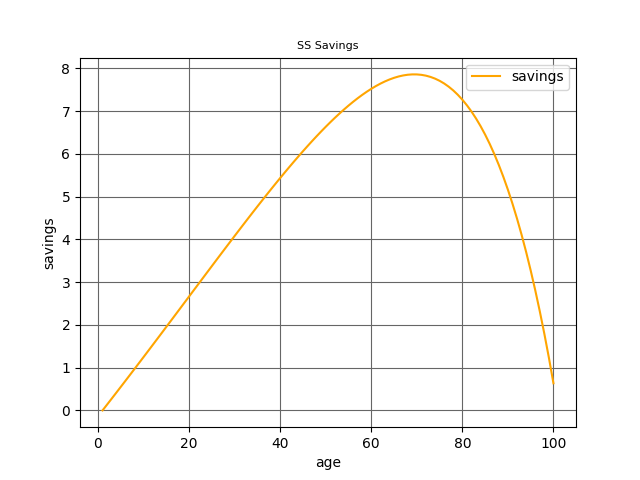
\includegraphics[width=5in]{savings.png}
		\caption{}
		\includegraphics[width=5in]{labour_supply.png}
		\caption{}
	\end{figure} 
    \begin{figure}
	\centering
	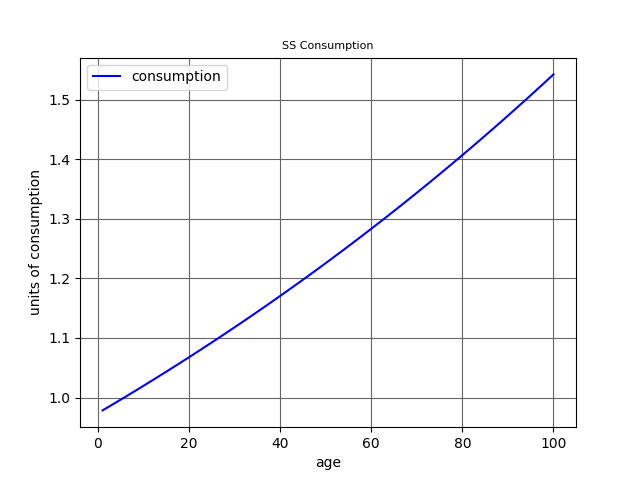
\includegraphics[width=5in]{consumption.png}
	\caption{}
    \end{figure} 

\end{document}